\section{Non-negative post-initialization}

%%%%%%%%%%%%%%%%%%%%%%%%%%%%%%%%%%%%%%%%%%%%%%%%%%%%%%%%%%%%%%%%%%%%%%%%%%%%%%%%%%%%%%%%%%%%%%%%%%%% 
\begin{frame}{Proposed Method}

  
  The proposed method can be applied on top of any existing initialization
  scheme.

  \begin{itemize}
  \item Unlocks the potential of non-negative neural networks
  \item Ensures high variance in the activation distribution
  \item Gradient propagation during the initial stage of training
  \item Increase the expressivity of the non-negative constrained models
  \end{itemize}
\end{frame}

% \begin{frame}{Novelties}
%     \begin{itemize}
%         \item The proposed framework allows one to apply it in traditionally used large architectures without any major change and performance degradation
%         \begin{itemize}
%             \item based on the non-negative isomorphic representation
%     of traditional models.
%         \end{itemize}
%         \item Investigates multiplicative updates in the context of non-negative training
%         \item Studying the isomorphism of the networks and proposing a structured methodology to acquire their nonnegative equivalent
%     \end{itemize}
% \end{frame}

\begin{frame}{On the Difficulty of Training Non-negative Neural Networks}
  % Conceptually, ANNs project the input features to a latent dimensional space,
  % aiming to represent them in a more separable way, seeking a hyperplane
  % decision boundary that can classify them in an optimal way. However,
  
\textbf{Classifying non-negative features}, even when they are linearly separable, is
  often \textbf{impossible when using non-negative parameters} for a linear classifier.

  \begin{equation}
    x_1 = - \frac{w_0}{w_1}x_0 - \frac{b}{w_1} \in \mathbb{R},
    \label{eq:reg_db}
  \end{equation}
  {\scriptsize where \(x_i \in [0, 1]\) is the input, \(w_i \in \mathbb{R}\)  and \(b\in
  \mathbb{R}\) are the weights and biases of the classifier, respectively, and
  \(i\in \{0, 1\}\). }

\begin{center}
	  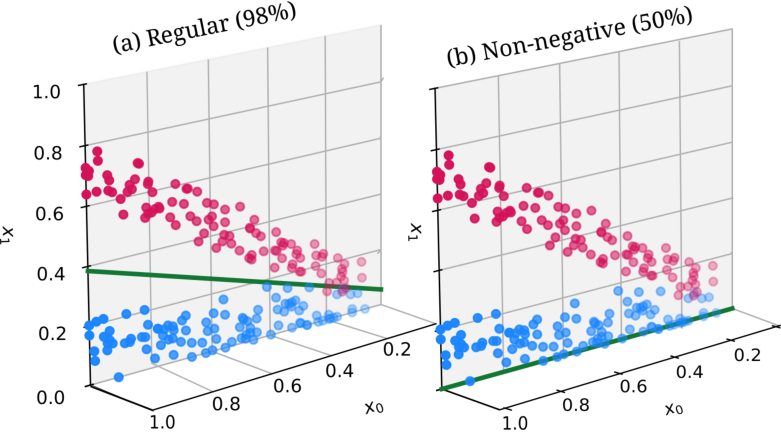
\includegraphics[width=0.6\textwidth]{sections/4_nn/imgs/training_issue.pdf}
\end{center}


  %  We can easily conclude that there is a positive slope decision, with the slope
  %  given by \(m=-w_{0}/w_{1}\), which requires a negative weight.

  %  \begin{itemize}
  % \item   In fact, training the linear classifier, using SGD, a positive slope decision
  % boundary is obtained achieving optimal performance with \(w_0<0\).
  % \item  On the other hand, constraining the classifier to
  % non-negative parameters results in a negative slope decision boundary that
  % cannot discriminate between the two classes
% \end{itemize}
\end{frame}

% \begin{frame}
  

% \end{frame}

% \begin{frame}{Isomorphism in Neural Networks}
% \textbf{Challenging computational tasks} can be easily solved by \textbf{changing the coordinate system}
% \begin{center}
%     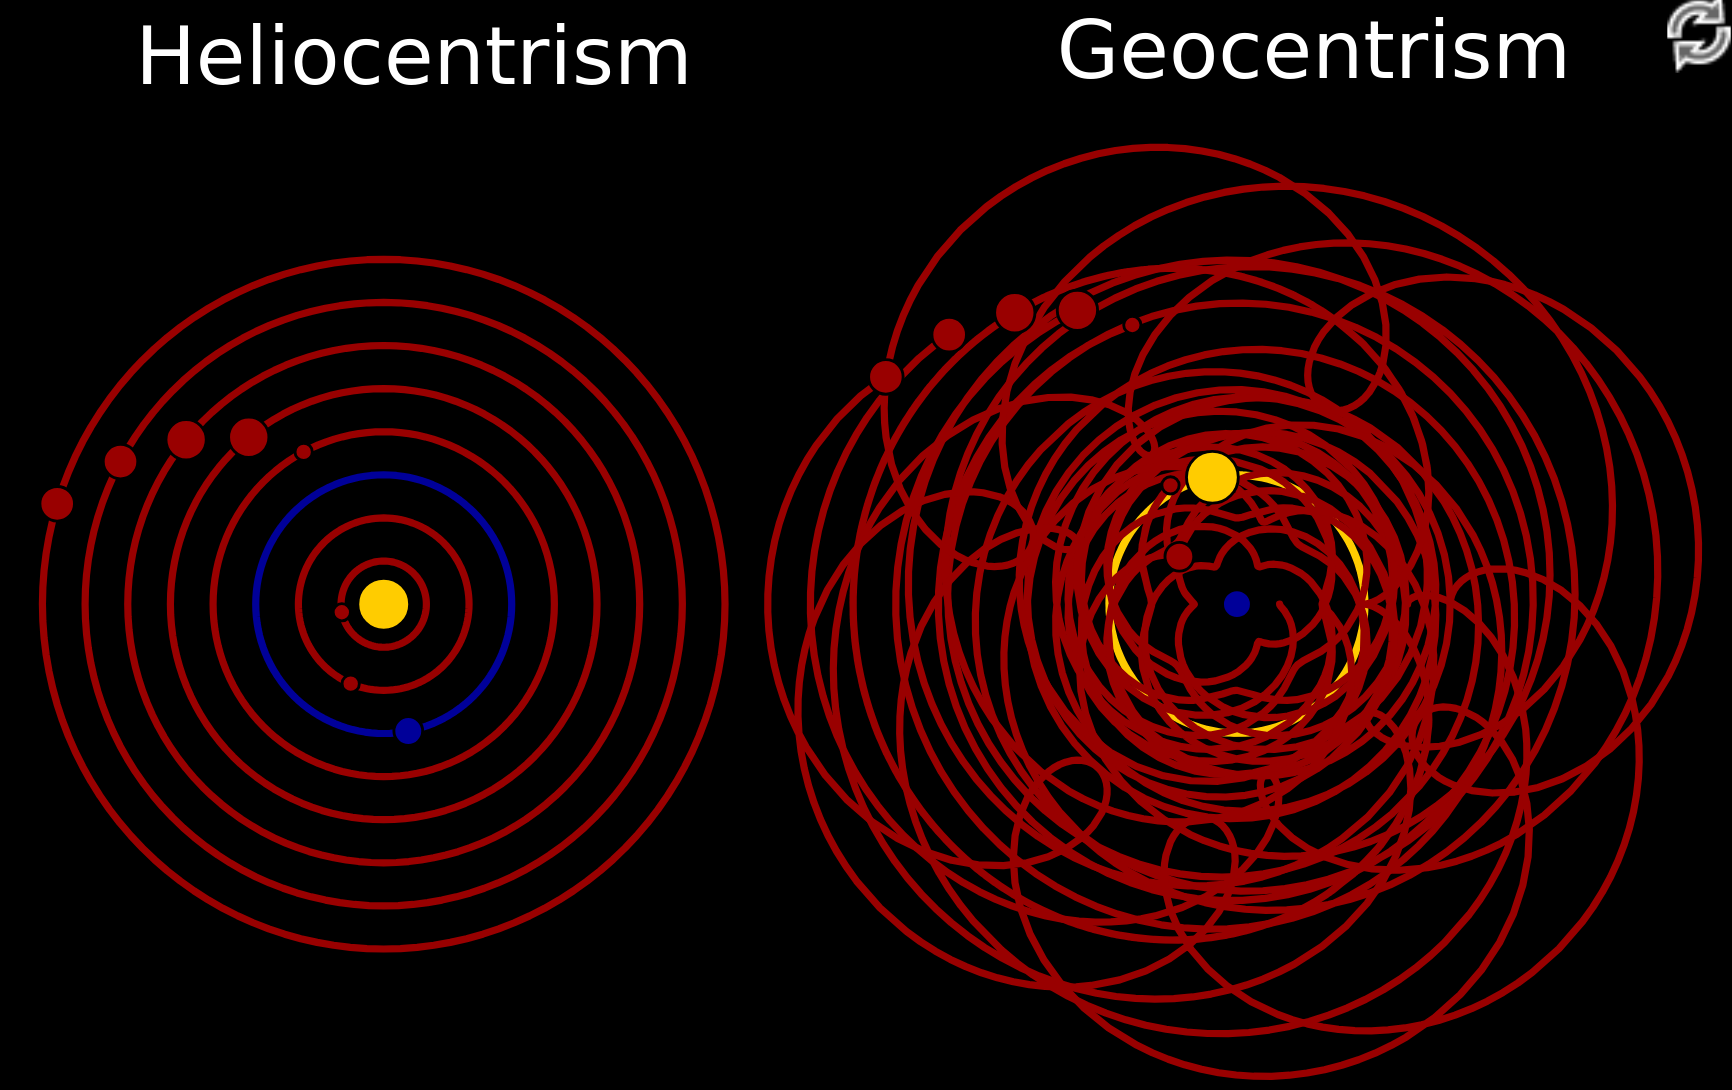
\includegraphics[width=0.45\textwidth]{sections/4_nn/imgs/Selection_548.png}
% \end{center}
% \textbf{Considering isomorphism}, it is claimed that \textbf{ an equivalent classifier with non-negative parameters exists}, producing the \textbf{same classification outcome as the original one.}
% \end{frame}

\begin{frame}{Transformation}

  \begin{columns}[T]
    \begin{column}{0.46\textwidth}
      The original task and classifier can be transformed, by \textbf{shifting
        and rotating the points and the decision boundary}, getting an
      equivalent non-negative classifier\textbf{, using only non-negative
        parameters.} The acquired non-negative classifier results in the decision boundary given by
      \begin{equation}
        x_1 =-\frac{\left|w_{0}\right|}{w_{1}} x_0' -\frac{b-a\left|w_{0}\right|}{w_{1}} \in \mathbb{R}
      \end{equation}
      {\scriptsize where \(w_0 < 0\), \(w_1 > 0\), \(a=1\) and
        \(x_0'=\left(a-x_0\right)\).}
      % The non-negative classifier leads to a rotated decision boundary and is equal to
      % the original classifier performance.
    \end{column}
    \begin{column}{0.46\textwidth}
      \begin{center}
        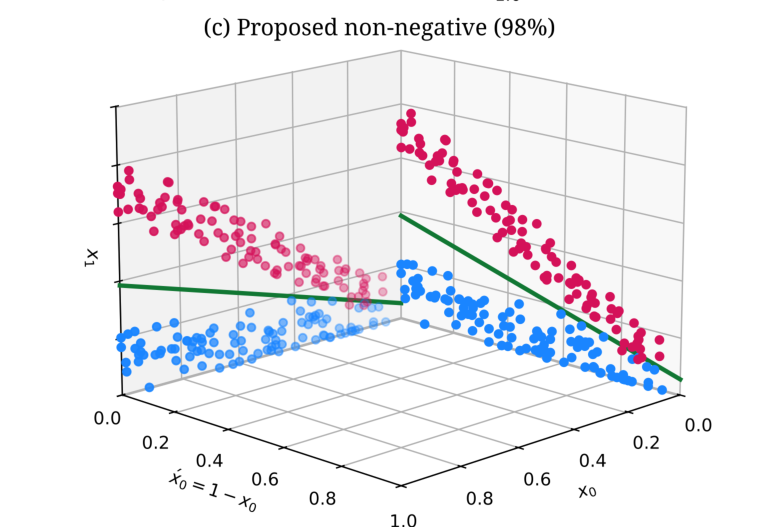
\includegraphics[width=\linewidth]{sections/4_nn/imgs/proposed_transformation.pdf}
      \end{center}

    \end{column}
  \end{columns}

  




\end{frame}

\begin{frame}{Definition of Fully-connected Layer}
  Let \(\bm{z}^{(j)} \in \mathbb{R}^{N_{j}}\) be the output of the linear part
  of the \(j\)-th layer of a neural network architecture, where the linear
  function is denoted as
  \(f^{(j)}(\cdot):\mathbb{R}^{N_{j-1}}\rightarrow\mathbb{R}^{N_{j}}\), given by 
  \begin{equation}
    \label{eq:linear}
    \bm{z}^{(j)} = f^{(j)}(\bm{x}^{(j)}) = \bm{W}^{(j)}\bm{x}^{(j)} + \bm{b}^{{(j)}} \in \mathbb{R}^{N_{j}},
  \end{equation}
  {\scriptsize where \(\bm{W}^{(j)} \in \mathbb{R}^{N_{j} \times  N_{j-1}}\),
    \(\bm{b}^{(j)} \in \mathbb{R}^{N_j}\), and \(\bm{x}^{(j)} \in
    \mathbb{R}^{N_{j-1}}\).}

  Assuming that an activation function \(\phi(\cdot): \mathbb{R}^{N_j} \rightarrow \mathbb{R}^{N_j}_{+}\), where \(\mathbb{R}_{+}\) denotes the set of positive real values, the output of the \(j\)-th layer is given by:
  \begin{equation}
    \label{eq:activation}
    \bm{y}^{(j)} = \phi^{(j)}(\bm{z}^{(j)}) \in \mathbb{R}^{N_j}_{+}.
\end{equation}
\end{frame}

% \begin{frame}{Definition Linear Neuron}
% Let \(z_i \in \mathbb{R}\) the \textbf{response of the linear part }of the \(i\)-th \textbf{neuron} of a fully connected
%   layer, where the linear function is denoted by \(u_{i}(\cdot): \mathbb{R}^{M}
%   \rightarrow \mathbb{R}\) and \(i = 1 \ldots N\), given by:  

%   \begin{equation}
%     \label{eq:linear_pass}
%     z_i = u_i(\bm{x}) = \sum_{j=1}^{M}{w_{ij}} x_j + b_i  \in \mathbb{R}, 
%   \end{equation}
%   {\scriptsize where \(\bm{w}_i \in \mathbb{R}^{M}\), \(b_i \in \mathbb{R}\) and \(\bm{x} \in
%   \mathbb{R}^{M}\) are the weight, bias, and input vectors of the \(i\)-th
%   neuron, respectively.}

%     Assuming an\textbf{ activation function }\(g(\cdot): \mathbb{R}
%   \rightarrow \mathbb{R}_{+} \), where \(\mathbb{R}_{+}\) denotes the set of
%   non-negative real values, the output of the \(i\)-th neuron is: 
%   \begin{equation}
%     y_i = g(z_i) \in \mathbb{R}_{+}.
%   \end{equation}

% \end{frame}

\begin{frame}{Transformation: Input Rotation}

\noindent
\begin{minipage}{.7\textwidth}
  Rotate the input multidimensional-space to a non-negative axis,
  projecting the weights that were originally initialized as negative onto the
  \begin{equation}
     \mathbbm{1}_{N_{j-1}}\alpha^{(j)} - \bm{x}^{(j)} \in [0,
  \alpha]^{{N_{j-1}}}-\text{axis}
  \end{equation}

  {\scriptsize with \(\mathbbm{1}_{N_{j-1}} \in [1, \ldots, 1]^{N_{j-1}}\) and \(\alpha^{(j)}
  \geq max(\mathcal{X}^{(j)})\) denotes the rotation constant of the layer  and
  \textit{max} denotes the maximum element in the feasible set \(\{x^{(j)}_{i} :
  \bm{x}^{(j)} \in [x_{min}, x_{max}]^{N_{j-1}} \subset
  \mathbb{R}_{+}^{N_{j-1}} \} \).}


  % . The , defined as \(\mathcal{X}^{(j)}\). The existence of the rotation constant \(\alpha^{(j)}\) requires a closed interval of \(\mathcal{X}^{(j)}\) that can be easily achieved in input through normalization or by considering a bounded activation function in the intermediate layers.
%       This allows us to \textbf{rotate} the \textbf{input feature space}, as
% \begin{equation*}
% \label{eq:rotated_input}
%     x_j' = f(x_j) = 
%     \begin{cases}
%         \alpha - x_j & \text{if } w_{ij} <  0\\
%         x_j     & \text{otherwise},
%     \end{cases}
% \end{equation*}
% {\scriptsize where \(x_j' \in \mathbb{R}_{+}\).} 
\end{minipage}% This must go next to `\end{minipage}`
\begin{minipage}{.3\textwidth}
    \begin{flushright}
    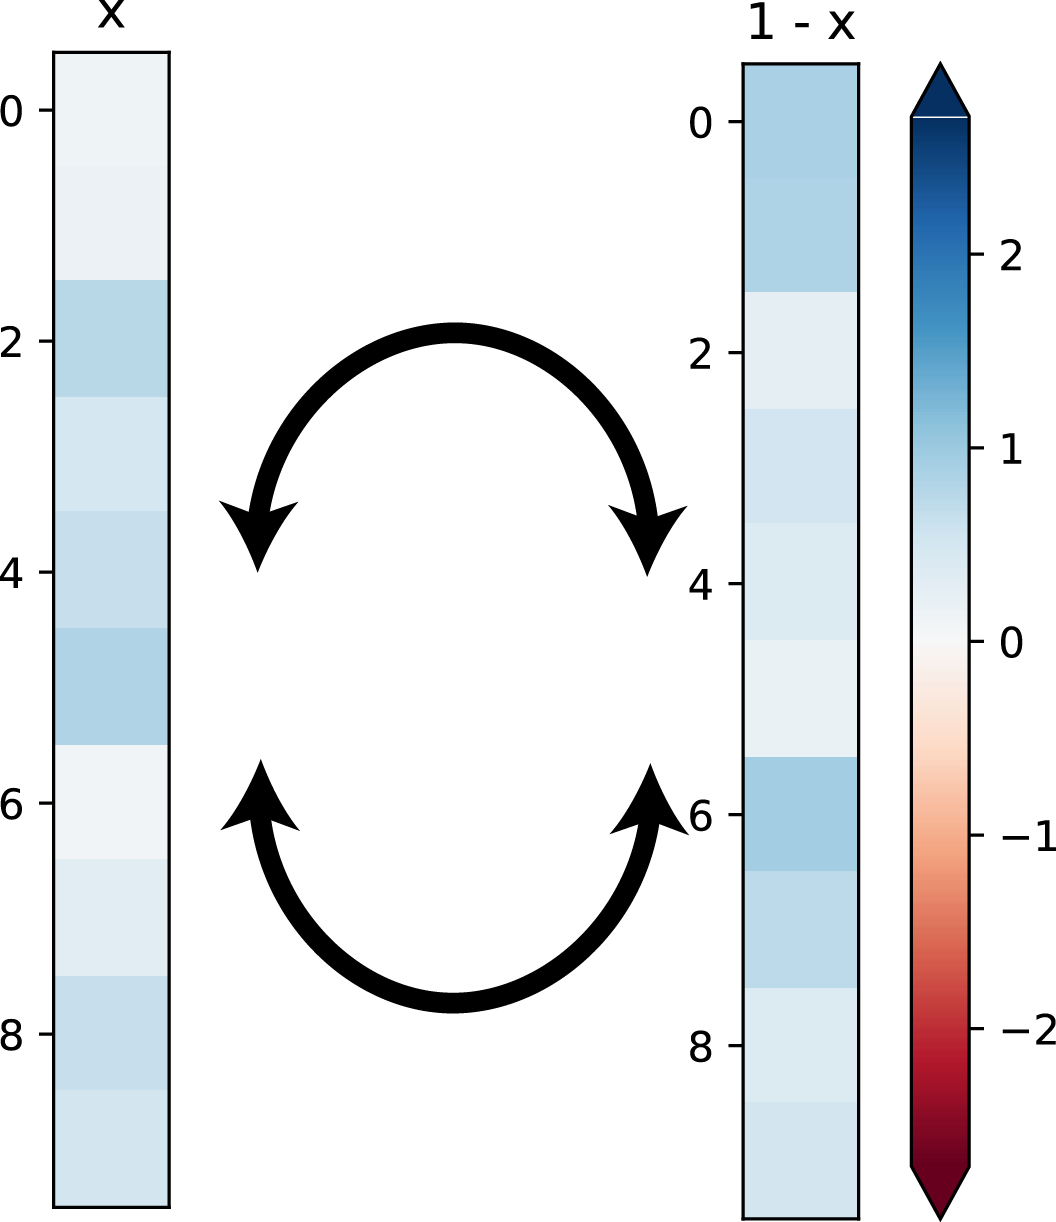
\includegraphics[width=0.8\linewidth]{sections/4_nn/imgs/x_1.png}
    \end{flushright}
\end{minipage}

\end{frame}


\begin{frame}{Transformation: Weight shifting}

  The initialized non-negative weights will retain their initial variance in those two axes as a projection
\begin{equation}
    \label{eq:trans_1}
    \bm{z}^{(j)} = \bm{W}_{-}^{(j)}(\mathbbm{1}_{N_{j-1}}\alpha^{(j)} - \bm{x}^{(j)}) + \bm{W}^{(j)}_{+}\bm{x}^{(j)} + \bm{b}^{'}{}^{(j)} \in \mathbb{R}_{+}^{N_j} 
\end{equation}
{\scriptsize where \(\bm{W}_{+}^{(j)} + \bm{W}_{-}^{(j)} = |\bm{W}^{(j)}|\) with
\(|\bm{W}^{(j)}| \in \mathbb{R_{+}}^{N_{j} \times N_{j-1}}\) denotes the
absolute value of the original weight matrix and \(\bm{b}^{'}{}^{(j)}\in
\mathbb{R}^{N_{j}}_{+}\) the bias vector. }

% \vspace{10pt}
% 	Linear neuron can be expressed as:
%   \begin{equation}
%     \label{eq:transformation_3}
%     z'_i = \sum_{\{j |w_{ij} < 0\}}|w_{ij}|(\alpha - x_{j}) + \sum_{\{j |w_{ij} > 0\}}w_{ij}x_j + \tilde{b}_i \in \mathbb{R}.
%   \end{equation} 

   \begin{center}
       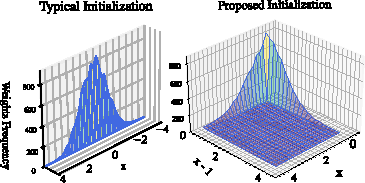
\includegraphics[width=0.6\linewidth]{sections/4_nn/imgs/wcci_proposal_v3.pdf}
   \end{center}

%  Both \(\bm{W}^{(j)}_{-} = \max(0,
% -\bm{W}^{(j)})\in \mathbb{R}_{+}^{N_{j} \times N_{j-1}}\) and \(\bm{W}_{+}=
% \max(0, \bm{W}^{(j)}) \in \mathbb{R}_{+}^{N_{j} \times N_{j-1}}\) are sparse
% matrices, each containing \(\approx 50 \%\) zero values.

 \end{frame}

 \begin{frame}{Transformation: Bias Integration}
   % The bias term can be initialized to any non-negative vector
   % \(\bm{b}^{'}{}^{(j)}\in \mathbb{R}^{N_j}_{+}\), however, this will lead to a
   % different variance in the output of the activation function, undermining the
   % applied initialization scheme.


   % To overcome this and ensure that the variance
   % of the activation values is preserved during training, we propose
   % initializing the biases based on the initialized weights and acquiring the
   % same variance in the activation distribution. More specifically, we propose
   % to accumulate

   The applied positive rotation of the weights in the
   \((\mathbbm{1}_{N_{j-1}}\alpha^{(j)} - \bm{x}^{(j)})\) axis is accumulated in the bias term
   and integrate it into a shifted activation function. Thus, the bias vector is
   initialized as  
   \begin{equation}
     \label{eq:new_bias}
     \bm{b}^{'}{}^{(j)} = \tilde{\bm{b}}^{(j)} + \mathbbm{1}_{N_{j}} c^{(j)} \in \mathbb{R}_{+}^{N_{j}},
   \end{equation}
   where
   \begin{equation}
     \label{eq:b_tilde}
     \tilde{\bm{b}}^{(j)} = \bm{b}^{(j)} - \sum_{i=0}^{N_j}\sum_{l=0}^{N_l} w^{(j)}_{il-} \in \mathbb{R}_{+}^{N_{j}},
   \end{equation}
   and \(c\in\mathbb{R}_{+}\) denotes the \textit{activation shifting point}
   computed as 
   \begin{equation}
     c^{(j)} = \max\{|b^{(j)}_0|, \ldots ,|b^{(j)}_{N_j}\} \in \mathbb{R}_{+} .
   \end{equation}

   \begin{center}
     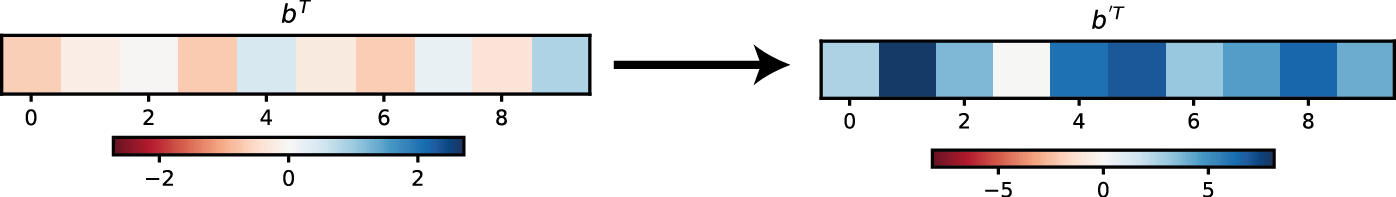
\includegraphics[width=0.9\linewidth]{sections/4_nn/imgs/bias.png}
   \end{center} \vspace{-10pt}
   
\end{frame}


% \begin{frame}{Transformation: Bias Integration}
% The last term can be \textbf{integrated} into an \textbf{updated bias}: 
% \begin{equation}
% \label{eq:bias_integration}
% \tilde{b}_i = b_i - \alpha\sum_{\{j |w_{ij} < 0\}}|{w}_{ij}| \in \mathbb{R}.
% \end{equation}

% The ne\textbf{w non-negative biases are transformed}:  
% \begin{equation}
% \label{eq:new_bias}
%     b^{'}_i = \tilde{b}_{i} + c \in \mathbb{R}_{+},
% \end{equation}
% with  \(c\in \mathbb{R}_{+}\) denotes \textbf{activation shifting point}
% \begin{equation}
%     c = \text{max}\{|\tilde{b}_0|, \ldots |\tilde{b}_{N}|\} \in \mathbb{R}_{+},
% \end{equation} 

% \begin{center}
%     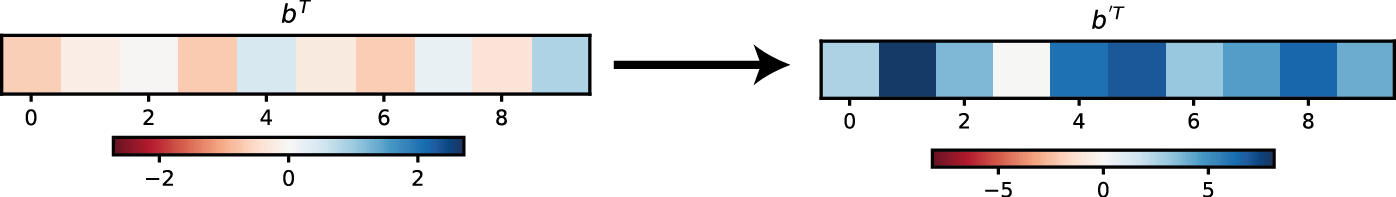
\includegraphics[width=0.9\linewidth]{sections/4_nn/imgs/bias.png}
% \end{center} \vspace{-10pt}

% \end{frame}

% The \textit{activation shifting point} is applied to the original activation to slide it into the input domain, preserving the variance of the original initialization scheme. To ensure that the network will function in a non-negative manner, the original activation function must operate within a closed interval with a non-negative output space, i.e., \(\phi^{(j)}(\bm{z}^{(j)}): \mathbb{R}^{N_{j}}\rightarrow [\phi^{(j)}_{min}, \phi^{(j)}_{max}]^{N_{j}}\), where \( 0 \leq \phi^{(j)}_{min} < \phi^{(j)}_{max} < \infty\), with the shifted activation calculated as:





\begin{frame}{Transformation: Activation Shifting Point}
The \textbf{activation shifting point} is applied \textbf{to the original activation},  \(\phi^{(j)}(\bm{z}^{(j)}): \mathbb{R}^{N_{j}}\rightarrow [\phi^{(j)}_{min}, \phi^{(j)}_{max}]^{N_{j}}\), where \( 0 \leq \phi^{(j)}_{min} < \phi^{(j)}_{max} < \infty\), to slide it into the input
domain, \textbf{leading to the same output as the original network}.
\begin{equation}
    \bm{y}^{(j)} = \phi^{(j)}_c(\bm{z}^{(j)})  = \phi^{(j)}(\bm{z}^{(j)} - \mathbbm{1}_{N_j} c^{(j)}) \in \mathbb{R}_{+}^{N_{j}}.
    \label{eq:nn_activation}
\end{equation}

\begin{center}
    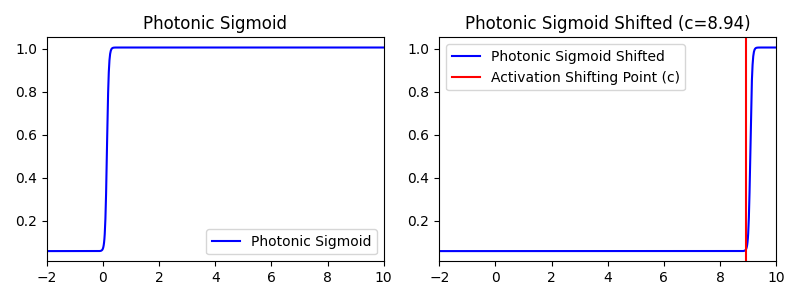
\includegraphics[width=0.8\linewidth]{sections/4_nn/imgs/sigmoid.png}
\end{center} 
\vspace{-10pt}
Typically, the \(\alpha^{(j+1)} \in \mathbb{R}_{+}\) of the next layer can be set to \(\alpha^{(j+1)} =
\phi^{(j)}_{max} = \text{max}(\mathcal{\bm{X}})\).      
\end{frame}

% \begin{frame}{Transformation: Non-negative Weights}

%   Similarly, the updated non-negative weights of the \(i\)-th neuron can be directly calculated as:
% \begin{equation}
%     \bm{w}'_{i} = |\bm{w}_i| \in \mathbb{R}_{+}^{M},
% \end{equation}
% % {\scriptsize where \(|\cdot|\) denotes the element-wise absolute value, i.e., \(w'_{ij} =
% % \{|w_{ij}|, j=0\ldots M\}\)}
% \begin{center}
%     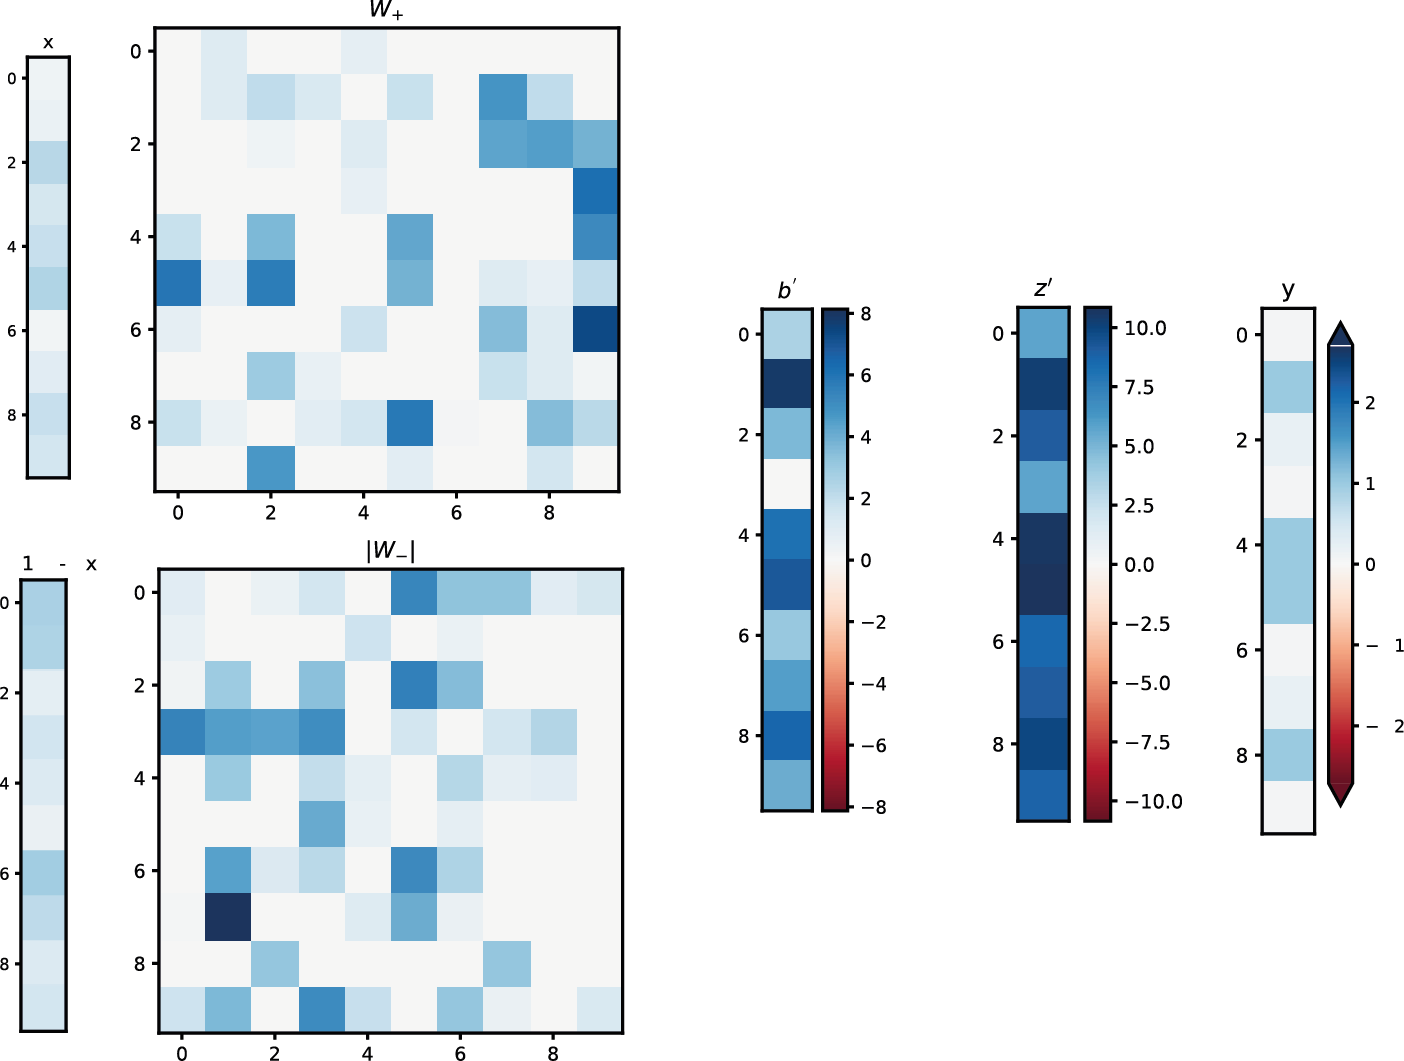
\includegraphics[width=0.7\linewidth]{sections/4_nn/imgs/overview_2.png}
% \end{center} 
    
% \end{frame}


% \begin{frame}{Non-negative Neuron}
% For \textbf{every linear neuron}, there is a \textbf{non-negative isomorphic} with the linear response provided as:
% \begin{equation}
%      z_i' = u_i'(\bm{x}')  =\sum_{j=1}^{M}|w_{ij}|x'_j + b'_i \in \mathbb{R}_+,
% \end{equation} and the output as: 
% \begin{equation}
%    y_i' = g_c(u_i'(\bm{x}')) \in \mathbb{R}_+,
% \end{equation} where:
% \begin{equation}
%     x'_j= 
%     \begin{cases}
%         \alpha - x_j & \text{if } w_{ij} <  0\\
%         x_j     & \text{otherwise}
%     \end{cases}.
% \end{equation}
% Then, the appropriate parameters \( b_i' \in \mathbb{R}_+ \) and \( \alpha \in \mathbb{R}_+ \), as well as the activation function \( g_c(\cdot): \mathbb{R} \rightarrow \mathbb{R}_+\) exist so that the neuron leads to the same response, i.e., \(y_i = y'_i\).
% \end{frame}

\begin{frame}{Post-initialization Remark}
	 Consider a linear layer followed by an activation function. defined by
   Equations~\ref{eq:linear} and~\ref{eq:activation}. Let the weights be
   initialized so that \(w_{ij} \sim \mathcal{D}(-a, a)\), and let the resulting
   activation distribution be denoted \(Y \sim \mathcal{A}(\mu, \sigma)\). 

    Given a post-initialization to non-negative weights \(\bm{W}^{'}=
    |\bm{W}|\), where \(\bm{W}_{+} + \bm{W}_{-} = |\bm{W}|\), there exist a
    corrective non-negative bias vector corrective \(\bm{b}^{'} \in
    \mathbb{R}_{+}^{N}\) and a shifted activation function \(\phi_c(\cdot):
    \mathbb{R}^{N} \rightarrow \mathbb{R}^{N}_{+}\) such that the new activation
    distribution \( Y^{'}\) satisfies \(Y^{'}\stackrel{d}{=}Y\). 
\end{frame}


\begin{frame}{Post-training Capability}
  \begin{figure}
\centering
    \begin{subfigure}{0.49\textwidth}
        \centering
        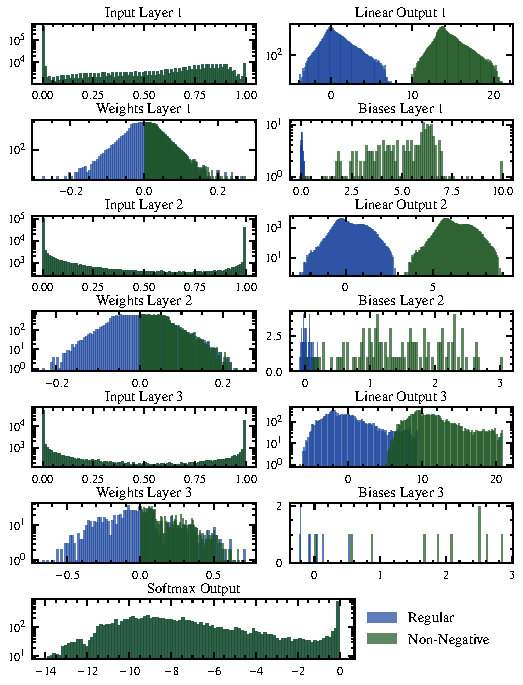
\includegraphics[width=0.8\textwidth]{sections/4_nn/imgs/transformation_plot.pdf}
    \end{subfigure}
    \hfill
    \begin{subfigure}{0.49\textwidth}
        \centering
        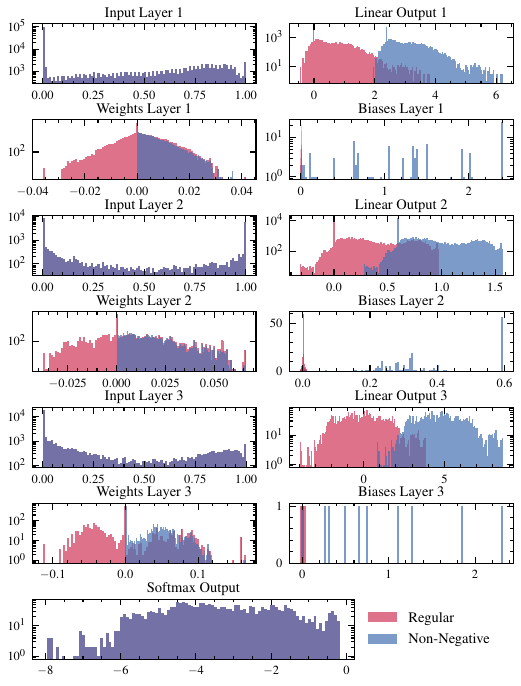
\includegraphics[width=0.8\textwidth]{sections/4_nn/imgs/variance_limited_range.png}
    \end{subfigure}
\end{figure}
\end{frame}


\begin{frame}{Generalibity}
  \begin{table}
    \begin{tabular}{l|c}
      Module                  & Covered \\
      \hline
      Recurrent Neuron        & $\checkmark$ \\
      Convolutional Neuron    & $\checkmark$ \\
      Padding                 & $\checkmark$ \\
      Negative Input          & $\checkmark$ \\
      Batch Normalization     & $\checkmark$ \\
      Residual Connection     & $\checkmark$ \\
    \end{tabular}
  \end{table}
\end{frame}

% \begin{frame}{Non-negative Stochastic Gradient Descent (NNSGD)}
% Transforming an already trained network to its non-negative isomorphic can be
%   \textbf{limiting in cases where continuing training is required.}
% \begin{equation}
% \small
% \theta_{\tau}^{(k)} = \theta_{\tau-1}^{(k)} +
% |\theta^{(k)}_{\tau-1}|\tanh{\left(-\eta_{in}\frac{\partial J}{\partial \theta^{(k)}_{\tau-1}} \right)} \eta_{out} \in \mathbb{R}^{+},
% \label{eq:3_m_abs}
% \end{equation}
% {\scriptsize where \(\eta_{in} \in \mathbb{R}^{+}\) is the inner and \(0 < \eta_{out} \leq
%   1\) the outer learning rate. } \\ \vspace{15pt}

% \textbf{NNSGD  modifies the additive update rule}, in which sign shifting is attributed
% during SGD optimization, by normalizing the gradients using the non-linear
% function \(\tanh: \mathbb{R} \rightarrow (-1, 1)\) and multiplying it by the
% absolute value of the parameter.  
% \end{frame}
\section{Evaluation Results}


\begin{frame}{Evaluation in Photonic Activations}
	\begin{table}
    \begin{center}
    \resizebox{0.85\linewidth}{!}{
    \begin{tabular}{l|l|lc|lc}
    % \toprule
      \multirow{2}{*}{Dataset} & \multirow{2}{*}{Architecture} & \multicolumn{2}{c|}{Photonic Sigmoid\footnote{\scriptsize P. Atanasijević, C. Pappas, et al,  Adaptive all-optical sigmoid activation functions for Photonic Neural Networks using Fabry-Perot laser diodes under optical injection, 2024 OFC }} & \multicolumn{2}{c}{Photonic Sinusoidal\footnote{\scriptsize N. Passalis, et al, Training Deep Photonic Convolutional Neural Networks With Sinusoidal Activations, 2021, IEEE TETCI}}\\
    \cline{3-6}
     && Proposed & \thead{Isomorphic\\Match} & Proposed & \thead{Isomorphic\\Match}\\
    \midrule
    MNIST & MLP & \(97.44\pm{0.08}\) & \checkmark & \(97.90\pm{0.10}\) & \checkmark\\ 
    MNIST & CNN & \(98.81\pm{0.14}\) & \checkmark & \(99.04\pm{0.07}\) & \checkmark \\
    FMNIST & MLP & \(85.64\pm{0.22}\) & \checkmark & \(86.30\pm{0.52}\) & \checkmark \\
    FMNIST & CNN & \(87.59\pm{0.47}\) & \checkmark & \(89.22\pm{0.18}\) & \checkmark \\
    CIFAR10 & MLP & \(37.08\pm{0.37}\) & \checkmark & \(39.48\pm{1.69}\) & \checkmark \\
    CIFAR10 & CNN & \(84.03\pm{0.69}\) & \checkmark & \(84.54\pm{0.28}\) & \checkmark \\
    Malimg\(^{*}\) & CNN & \(91.06\pm{4.56}\) & \checkmark & \(93.28\pm{4.30}\) & \checkmark \\
    Names & RNN & \(56.02\pm{0.70}\) & \checkmark & \(65.82\pm{0.90}\) & \checkmark \\
    FI2010\(^{\dagger}\) & RNN & \(0.1371\pm{0.0024}\) & \checkmark & \(0.1612\pm{0.0033}\)& \checkmark \\
    % \bottomrule
    \end{tabular}}
    \end{center}
    \vspace{-3pt}
    \scriptsize{\({*}\)F1 score, \({\dagger}\)Cohen's kappa score are reported, since the datasets are highly unbalanced}
\end{table}
\end{frame}

\begin{frame}{Evaluation on traditional (CNN Architectures)}
\begin{table}
  \begin{tabular}{lc|cc|cc|c}
    \multirow{2}{*}{\textbf{Architecture}} & \multirow{2}{*}{$\alpha$} &  \multicolumn{2}{c|}{\textbf{Original}} & \multicolumn{2}{c|}{\textbf{Isomorphic}} & \multirow{2}{*}{$ \mathbf{\leq0.5\%} $}\\
                 &          & \textbf{Acc@1} & \textbf{Acc@5} & \textbf{Acc@1} & \textbf{Acc@5} & \\
    \hline
    \textbf{AlexNet} & 25 & 56.52 & 79.06 & 56.36 & 79.10 & \checkmark\\
    \textbf{VGG11} & 25 & 69.02 & 88.62 & 68.95 & 88.59 & \checkmark\\
    \textbf{VGG13} & 40 & 69.93 & 89.25 & 69.83 & 89.28 & \checkmark\\
    \textbf{VGG16} & 100 & 71.59 & 90.38 & 71.59 & 90.40 & \checkmark\\
    \textbf{VGG19} & 100 & 72.37 & 90.87 & 72.39 & 90.90 & \checkmark\\
    \textbf{ResNet18} & 25 & 69.75 & 89.08 & 69.76 & 89.08 & \checkmark\\
    \textbf{ResNet34} & 25 & 73.31 & 91.42 & 73.29 & 91.42 & \checkmark\\
    \textbf{ResNet50} & 100 & 80.85 & 95.43 & 80.35 & 95.13 & \checkmark\\
    \textbf{ResNet101} & 100 & 81.88 & 95.78 & 81.67 & 95.66 & \checkmark\\
    \textbf{ResNet152} & 100 & 82.28 & 96.00 & 82.34 & 95.34 & \checkmark\\
  \end{tabular}
\end{table}
\end{frame}

% \begin{frame}{Post-training Variance Study}
%   \begin{figure}
%     \centering
%     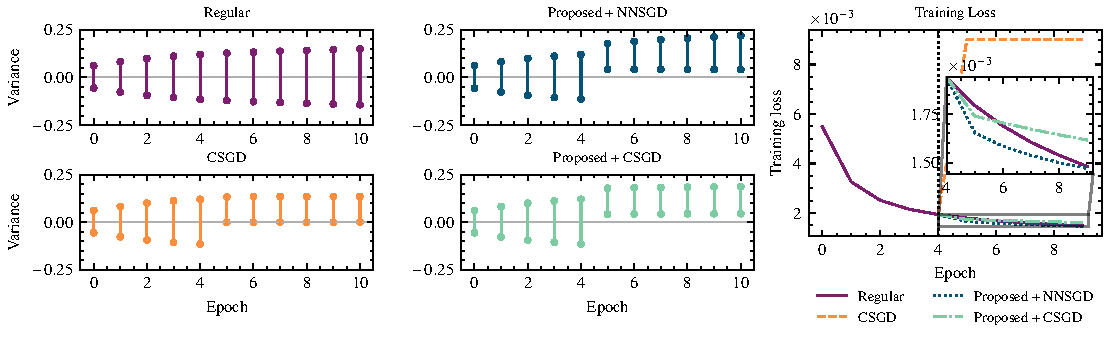
\includegraphics[width=\linewidth]{sections/4_nn/imgs/variance_fmnist_photonic_sigmoid.pdf}
%     % \vspace{-25pt}
%     \caption{Depicts the variance of classification layer in photonic sigmoid architecture applied on FMNIST dataset. Additionally, in the right subfigure, the loss during the training is presented. Networks are pre-trained for 5 epochs with SGD and then they are either transformed with the proposed method or clipping is applied directly. The figure in the top left shows the variance of the regular training. }
%     \label{fig:fmnist_variance}
%     % \vspace{-15pt}
% \end{figure}
% \end{frame}


% \begin{frame}{Non-negative Post-training (MLPs)}
%    \begin{table}[]
%     \centering
%      \caption{Non-negative post training after transformation using MLPs}  
%       \label{tab:3_half_fcnn}
%     \begin{tabular}{l|ll|l}
%          % \toprule
%          Dataset  & \thead{Regular\\+ CSGD} & \thead{Proposed\\+ CSGD} &  \thead{Proposed\\+ NNSGD}  \\
%          \midrule
%          \multicolumn{4}{c}{Photonic Sigmoid}\\
%          \midrule
%          MNIST  & \(11.00\pm{0.00}\) & \(\bm{97.31\pm{0.90}}\) & \(\underline{\bm{97.40\pm{0.06}}}\) \\
%          FMNIST & \(10.00\pm{0.00}\) & \(\bm{84.77\pm{0.21}}\) & \(\underline{\bm{85.01\pm{0.12}}}\) \\
%          CIFAR10 & \(10.00\pm{0.00}\) & \(\bm{36.34\pm{0.37}}\) & \(\underline{\bm{36.81\pm{0.33}}}\)\\
%          \midrule
%          \multicolumn{4}{c}{Photonic Sinusoidal}\\
%          \midrule
%          MNIST  &  \(09.74\pm{0.00}\)  & \(\bm{97.85\pm{0.10}}\) & \(\underline{\bm{97.86\pm{0.07}}}\) \\
%          FMNIST  & \(10.00\pm{0.00}\) & \(\bm{86.62\pm{0.09}}\) & \(\underline{\bm{86.95\pm{0.17}}}\)\\
%          CIFAR10 & \(10.00\pm{0.00}\) & \(\bm{40.96\pm{0.30}}\) & \(\underline{\bm{41.19\pm{0.38}}}\)\\
%          % \bottomrule
%     \end{tabular}
% \end{table}
% \end{frame}

% \begin{frame}{Non-negative Post-training (CNNs \& RNNs)}
% 	\begin{table}
% \caption{Non-negative post training after transformation using CNNs and RNNs \label{tab:half}}
%     \begin{center}
%     \resizebox{\linewidth}{!}{
%     \begin{tabular}{l|ll|ll}
%     % \toprule
%         Config.& \multicolumn{2}{|c|}{Photonic Sigmoid}  & \multicolumn{2}{|c}{Photonic Sinusoidal}\\
%         \midrule
%         Method  & \thead{Proposed\\+ CSGD} & \thead{Proposed\\+ NNSGD} & \thead{Proposed\\+ CSGD} & \thead{Proposed\\+ NNSGD}  \\
%         \midrule
%         MNIST & \(96.85\pm{0.96}\) & \(\bm{97.60\pm{1.83}}\) & \(98.58\pm{0.12}\) & \(\bm{99.04\pm{0.07}}\) \\
%         FMNIST & \(83.90\pm{0.46}\) & \(\bm{84.87\pm{0.33}}\) & \(87.59\pm{0.20}\) &  \(\bm{87.63\pm{0.19}}\) \\
%         CIFAR10 & \(74.30\pm{0.22}\) & \(\bm{77.39\pm{0.56}}\) & \(77.30\pm{0.73}\) & \(\bm{79.95\pm{0.21}}\) \\
%         Malimg\(^{*}\) & \(93.53\pm{2.76}\) & \(\bm{96.60\pm{0.78}}\) & \(92.18\pm{4.52}\) & \(\bm{93.53\pm{4.30}}\) \\
%         \midrule
%         Names & \(53.94\pm{1.44}\) & \(\bm{58.37\pm{1.05}}\) &  \(66.64\pm{0.83}\) & \(\bm{67.14\pm{0.54}}\) \\
%         FI2010\(^{\dagger}\) & \(0.1050\pm{0.0070}\) & \(\bm{0.1220\pm{0.0022}}\) & \(0.1434\pm{0.0014}\)  & \(\bm{0.1840\pm{0.0018}}\) \\
%         % \bottomrule
%     \end{tabular}}
%      \end{center}
%      \vspace{-3pt}
%     \scriptsize{\({*}\)F1 score, \({\dagger}\)Cohen's kappa score are reported, since the datasets are highly unbalanced}
%     \vspace{-10pt}
% \end{table}
% \end{frame}



% \begin{frame}{Non-negative Training from Scratch (MLPs)}
% 	\begin{table}[]
%     \centering
%          \caption{Non-negative training from scratch in MLPs}  
%       \label{tab:full_fcnn}
%     \resizebox{\linewidth}{!}{
%     \begin{tabular}{l|ll|ll}
%          \toprule
%          Dataset  & \thead{Exp. Initialization\\+ CSGD} & \thead{Proposed\\+ CSGD} & \thead{Exp. Initialization\\+ NNSGD} & \thead{Proposed\\+ NNSGD}  \\
%          \midrule
%          \multicolumn{5}{c}{Photonic Sigmoid}\\
%          \midrule
%          MNIST & \(11.35\pm{0.00}\) &\(\bm{92.52\pm{0.52}}\) & \(11.35\pm{0.00}\) & \(\underline{\bm{93.34\pm{1.11}}}\) \\
%          FMNIST & \(10.00\pm{0.00}\) &\(\bm{82.31\pm{1.29}}\) & \(10.00\pm{0.00}\) & \(\underline{\bm{84.09\pm{0.56}}}\)\\
%          CIFAR10 & \(10.00\pm{0.00}\) &\(\bm{37.25\pm{1.57}}\)  & \(10.00\pm{0.00}\) & \(\underline{\bm{37.61\pm{1.76}}}\)\\
%          \midrule
%          \multicolumn{5}{c}{Photonic Sinusoidal}\\
%          \midrule
%          MNIST  & \(86.36\pm{1.39}\) &\(\bm{92.51\pm{0.78}}\) & \(35.31\pm{6.11}\) & \(\underline{\bm{94.14\pm{0.90}}}\)\\
%          FMNIST & \(68.95\pm{3.71}\) &\(\bm{82.91\pm{0.55}}\)   & \(9.97\pm{0.02}\) & \(\underline{\bm{83.57\pm{0.26}}}\)\\
%          CIFAR10 &  \(10.00\pm{0.00}\) &\(\bm{34.96\pm{2.44}}\) & \(10.00\pm{0.00}\)  & \(\underline{\bm{35.41\pm{1.43}}}\)\\ 
%          \bottomrule
%     \end{tabular}}
%   \end{table}
%   \end{frame}

% \begin{frame}{Non-negative Training from Scratch (CNNs \& RNNs)}
%   \begin{table}[]
%    \caption{Non-negative training from scratch in CNNs and RNNs \label{tab:full}} 
%     \begin{center}
%     \resizebox{\linewidth}{!}{
%     \begin{tabular}{l|ll|ll}
%     \toprule
%         Config.& \multicolumn{2}{|c|}{Photonic Sigmoid}  & \multicolumn{2}{|c}{Photonic Sinusoidal}\\
%         \midrule
%         Method  & \thead{Proposed\\+ CSGD} & \thead{Proposed\\+ NNSGD} & \thead{Proposed\\+ CSGD} & \thead{Proposed\\+ NNSGD}  \\
%         \midrule
%         MNIST & \(97.69\pm{0.20}\) & \(\bm{98.14\pm{0.23}}\) & \(98.54\pm{0.14}\) & \(\bm{98.71\pm{0.05}}\) \\
%         FMNIST & \(83.81\pm{0.85}\) & \(\bm{83.87\pm{0.19}}\) & \(87.77\pm{0.36}\) & \(\bm{87.86\pm{0.36}}\)\\
%         CIFAR10 & \(71.61\pm{1.04}\) & \(\bm{72.16\pm{0.54}}\) & \(69.87\pm{1.73}\) & \(\bm{75.16\pm{1.83}}\)\\
%         Malimg\(^{*}\) & \(91.47\pm{4.37}\) & \(\bm{91.98\pm{4.00}}\) & \(96.53\pm{0.42}\) & \(\bm{97.26\pm{0.31}}\) \\
%         \midrule
%         Names & \(54.00\pm{2.13}\) & \(\bm{56.68\pm{1.11}}\) & \(64.17\pm{0.14}\) & \(\bm{68.70\pm{0.78}}\) \\
%         FI2010\(^{\dagger}\) & \(0.1338\pm{0.0045}\) & \(\bm{0.1498\pm{0.0112}}\) & \(0.1732\pm{0.0175}\) & \(\bm{0.1789\pm{0.0102}}\)\\
%         \bottomrule
%     \end{tabular}}
%      \end{center}
%      \vspace{-3pt}
%     \scriptsize{\({*}\)F1 score, \({\dagger}\)Cohen's kappa score are reported, since the datasets are highly unbalanced.}
% \end{table}
% \end{frame}

% \begin{frame}{Publication}
% \begin{itemize}
%     \item Main Journal Submission
%     \begin{itemize}
%         \item {\scriptsize \textbf{Kirtas, M.}, Passalis, N., Pleros, N., Tefas, A., 2024. \href{https://arxiv.org/abs/2310.01084}{Non-Negative Isomorphic Neural Networks for Efficient Accelerators.} \textbf{Submitted}}
%     \end{itemize}
%     \item Main Conferences Publications 
%         \begin{itemize}
%         \item {\scriptsize \textbf{Kirtas, M.}, Tsampazis, K., Avramelou, L., Passalis, N. and Tefas, A., 2023, September. \href{https://link.springer.com/chapter/10.1007/978-3-031-74627-7_35}{Using Part-based Representations for Explainable Deep Reinforcement Learning.} In Joint European Conference on Machine Learning and Knowledge Discovery in Databases}
%     \end{itemize}
% \end{itemize}
% \end{frame}
